%%
% This is an Overleaf template for scientific articles and reports
% using the TUM Corporate Desing https://www.tum.de/cd
%
% For further details on how to use the template, take a look at our
% GitLab repository and browse through our test documents
% https://gitlab.lrz.de/latex4ei/tum-templates.
%
% The tumarticle class is based on the KOMA-Script class scrartcl.
% If you need further customization please consult the KOMA-Script guide
% https://ctan.org/pkg/koma-script.
% Additional class options are passed down to the base class.
%
% If you encounter any bugs or undesired behaviour, please raise an issue
% in our GitLab repository
% https://gitlab.lrz.de/latex4ei/tum-templates/issues
% and provide a description and minimal working example of your problem.
%%


\documentclass[
  english,        % define the document language (english, german)
  font=times,     % define main text font (helvet, times, palatino, libertine)
  onecolumn,      % use onecolumn or twocolumn layout
]{tumarticle}


% load additional packages
\usepackage{lipsum}


% article metadata
\title{Time stepping review of open-source solvers}
\subtitle{Guided research}

\author[email=marc.amoros@tum.de]{Marc Amorós}

\date{
    \small
    \textbf{Advisor:} M.Sc. Benjamin Rodenberg \\
    \textbf{Supervisor:} Prof. Dr. Hans-Joachim Bungartz \\
}

\begin{document}

\maketitle

% \begin{abstract}
%   This is a short abstract summarizing the main points of your article.
% \end{abstract}

\section{Introduction}
\begin{itemize}
    \item Introduction to coupling simulations (FSI) and to the preCICE library. 
    \item Some brief motivation of performing a convergence study on the known solvers.
    \item Talk somehow about higer timestepping schemes, and why/when is good to use them. Should you use a higher order timestepping scheme if it doesn't give good results? (No bc it is slower) 
    \item Say why we chose this two open source solvers.
    \item Explain difference between preCICEv2 and preCICEv3.
\end{itemize}


\section{OpenFOAM}
\begin{itemize}
    \item Small introduction to OpenFOAM.
    \item Explain time stepping schemes available in the solver, and their orders. Mainly talk about Euler method, and Crank Nikolson, as they are the two cases we used.
    \item Talk about the script created to automatize the procedure of running these simulations. 
\end{itemize}

\subsection{Solver parameters}
\begin{itemize}
    \item Talk about the important parameters in the configuration, to obtain accurately enough results, as those where quite time consuming to find. For example, foamToVTK is not accurate enough, and was misleading at the beginning. Also mention the solver used.
\end{itemize}

\subsection{Case study: Taylor Green Vortex}
\begin{itemize}
    \item Short introduction to the scenario, present generation formulas of initial conditions and boundary conditions.
    \item Explain how the error is computed, while commenting Figure \ref{fig:error_x_y}.
\end{itemize}

\begin{figure}[!ht]
    \centering
    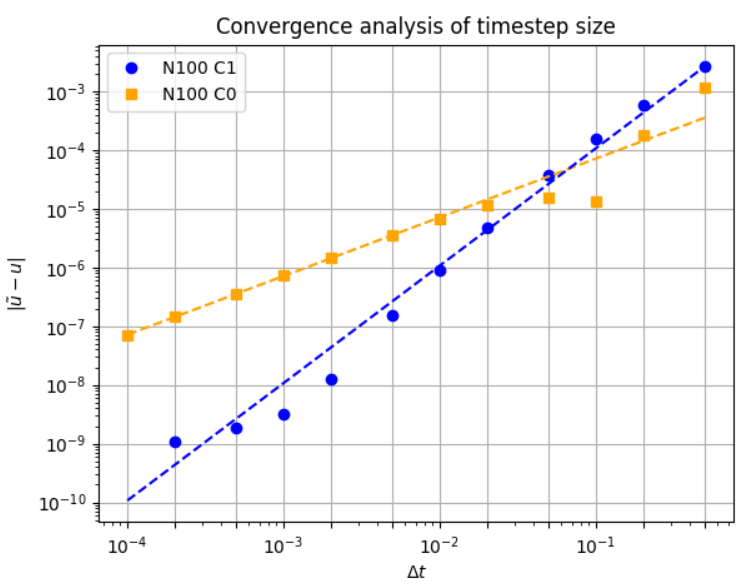
\includegraphics[width=0.5\textwidth]{resources/convergence_study_N100.PNG}
    \caption{Figure comparing data to the analytical solution of Taylor green vortex.}
    \label{fig:error_x_y}
\end{figure}

\begin{itemize}
    \item Talk about the second way of computing the error, while commenting Figure \ref{fig:RMSE}. Talk about the appearence of the spatial discretization error, and at which scales happens.
\end{itemize}

\begin{figure}[!ht]
    \centering
    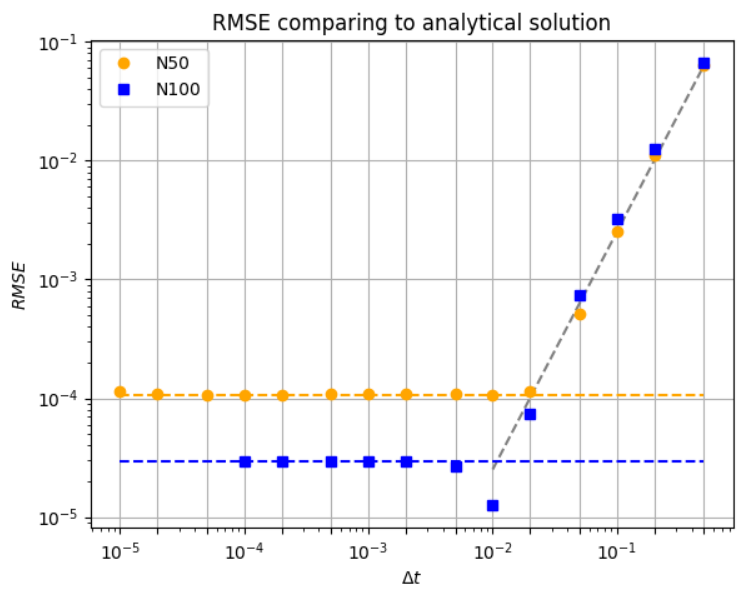
\includegraphics[width=0.5\textwidth]{resources/RMSE_study.PNG}
    \caption{Figure showing spatial error decrease with higher grid definition. TODO: improve this figure, as you computed also with N150.}
    \label{fig:RMSE}
\end{figure}

\section{Calculix}
\begin{itemize}
    \item Small introduction to Calculix.
    \subsection{Solver parameters}
    \item Talk about the supported time stepping scheme (only one, but higher order). In this case the parametrization is quite simpler, so I would also summarize it here.
    
    \subsection{Case study: perpendicular flap}
    \item Talk about the simulation that we performed, a perpendicular flap versus a constant force.
    \item Mention the scripts created to automatize this task, and to obtain the tip point value from the results.
    \item Comment on Figure \ref{fig:calculix_convergence}, that shows a higher order (between 1 and 2) of convergence. Mention how we compute the error, and how for values <1e-4 the outputed value is the same, meaning either that for lower timesteps the spatial discretization error governs, or that the solver can't achieve better accuracy bc of how values are stored (max of 6 decimal values, more likely given that the results are the exact same). 
    
    \begin{figure}
        \centering
        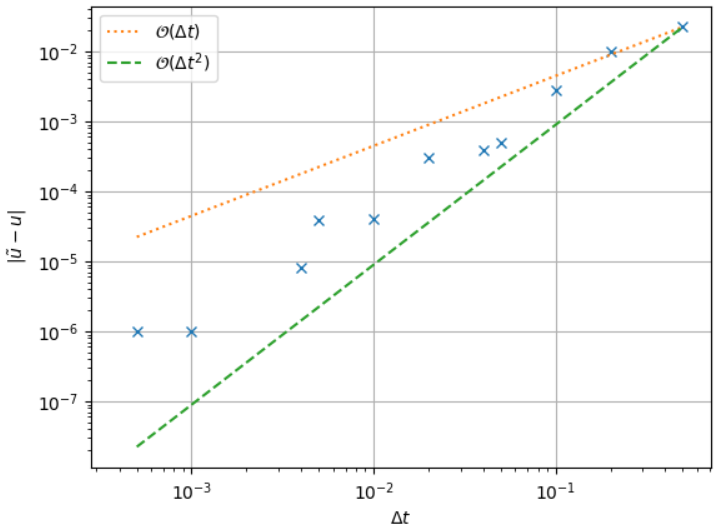
\includegraphics[width=0.5\textwidth]{resources/calculix_convergence_study.png}
        \caption{TODO: improve this figure, by adding legend and nicer colors.}
        \label{fig:calculix_convergence}
    \end{figure}

\end{itemize}

\section{Coupling the two solvers}
\begin{itemize}
    \item Talk about what a FSI is in general. Talk more specifically about the perpendicular flap case study, based on the preCICE tutorials.
    \item Talk about the automatization of this, using scripts.
    \item Supported time stepping schemes, difference between v2 and v3.
\end{itemize}
\subsection{Simulation parameters}
    \begin{itemize}
    \item Talk about the parameters of the two solvers (mainly the same as the previous simulations, except change of openFAOM solver). 
    \item Mention the possible preCICE parameters (window-size, ...).
    \end{itemize} 

\subsection{Case study: FSI - perpendicular flap}
\begin{itemize}
    \item Comment on Figure \ref{fig:coupled_v2_v3}. Show how First order convergence seems to be working, but higher order performs poorly. This is due to an error on the openFAOM adapter, which only supports Euler timestepping.
    \item Crank Nikolson needs two evaluations per time step, or reuse buffered data of previous timesteps (what is doing openFAOM, most likely, TODO: check this.).
    \item Give reasoning why this is not working, give some clues what should be done to actually improve it.
\end{itemize}


\begin{figure}[!ht]
    \centering
    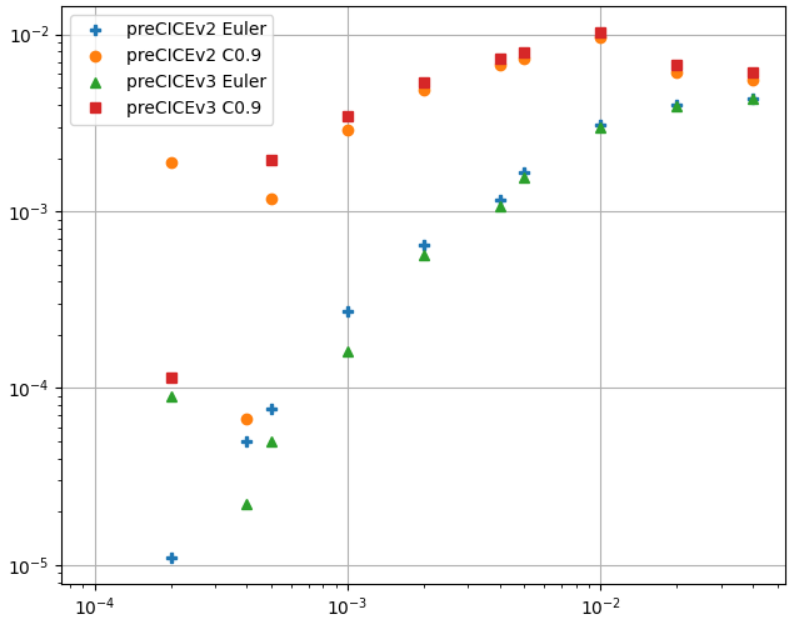
\includegraphics[width=0.5\textwidth]{resources/coupled_v2_v3_results.PNG}
    \caption{TODO: add title and maybe convergence lines}
    \label{fig:coupled_v2_v3}
\end{figure}


\section{OpenFOAM Adapter}
\begin{itemize}
    \item Maybe explain a bit how it interacts with the solver, quite documented already by \href{https://precice.org/adapter-openfoam-extend.html}{Adapter documentation}, and by \href{https://journal.openfoam.com/index.php/ofj/article/view/88/78}{Article of Gerasimos et al.}.
    \item Mention what should be fixed, maybe propose a prototype?
    \item Mention how should be tested, with a fake-fluid setup for example. Then also test with the same setup to see if it is viable.
\end{itemize}

\section{Conclusions and future work}
\begin{itemize}
    \item Talk about the convergence conclusions of each of the solvers. Mention the obtained results with the preCICE couplings.
    \item Give directions on what to fix of the OpenFOAM adapter, and what to be tested after the fixing implementation.
     
\end{itemize}


\end{document}
